\begin{exercise}{Dynamo}{-1}{Spé}
{}{mines}

\paragraph{Question de cours}~

Mesure d'une enthalpie standard de réaction par calorimétrie.

\paragraph{Exercice}~

On considère le dispositif suivant composé d'un cylindre conducteur en rotation à la vitesse angulaire $\Omega$  et soumis à un frottement visqueux $\alpha$ (en haut), relié à un système de spires de résistance totale $R$ et d'inductance $L$ parcourues par un courant $I$ générant un champ magnétique $\vec{B}$ supposé uniforme au niveau du disque (en bas).

\begin{center}
    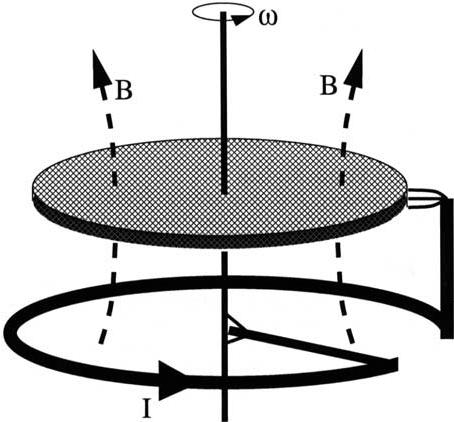
\includegraphics[width=.5\linewidth]{oraux/mines/bullard-dynamo.png}
\end{center}

On considère tout d'abord que le courant $I$ du système est constant.

\begin{questions}
\question Exprimer le lien entre le champ $B$ au niveau de la spire et le courant $I$.
\question Justifier l'existence d'une force de Laplace au niveau du cylindre. En déduire l'équation de la dynamique du système et montrer que la vitesse de rotation $\Omega$ du système croît jusqu'à une valeur limite en un temps $\tau$ qu'on précisera tous deux.
\uplevel{On fixe maintenant la vitesse de rotation $\Omega$, mais le courant $I$ n'est plus constant.}
\question En notant $e$ la force électromotrice induite dans le circuit, établir l'équation de la dynamique électrique du circuit.
\question Par un argument énergétique, déterminer la valeur de $e$.
\question Montrer que au dessus d'une vitesse de rotation seuil $\Omega_c$, le courant dans le système croit exponentiellement. En quoi cela est surprenant ?
\end{questions}

% \begin{questions}
% \question Donner l'expression de la force de Laplace exercée par le champ magnétique sur le cylindre. Quel est son effet d'un point de vue dynamique ?
% \question En déduire l'équation de la dynamique mécanique du système et montrer que la vitesse de rotation $\Omega$ du système croit jusqu'à une valeur limite en un temps $\tau$ qu'on précisera tout deux.
% \uplevel{Le champ magnétique $B$ et le courant $I$ ne sont toutefois pas constants.}
% \question Décrire qualitativement ce qu'il se passe d'un point de vue du circuit électrique.
% \question En notant $e$ la force électromotrice induite dans le circuit électrique, établir l'équation de la dynamique électrique du circuit.
% \question En justifiant qualitativement que $e = \Omega M I$ (on précisera la significationet l'unité de $M$), montrer que pour $\Omega$ constant et au dessus d'un certain seuil $\Omega_c$ (dont on donnera l'expression), le courant dans le système croit exponentiellement. En quoi cela est surprenant ?
% \question Effectuer les bilans énergétiques électrique, mécanique et total du système, en interprétant chaque terme.
% \question En déduire un lien entre $M$, $L$, $I$, $B$ et $R$.
% \end{questions}

\end{exercise}

\begin{solution}
    \begin{questions}
        \question $\dd{\vec{F}}_\textsc{l} = I\dd{\vr}\cross\vB = -I B \dd{r}\ve_\theta$. La force de Laplace a pour effet de faire tourner le système.
        \question On uilise donc le TMC. Le couple des forces de laplace est
        $$\vec{\Gamma}_\textsc{l} = \int\vr\cross(I\dd{\vr}\cross\vB) = -I B \int r\dd{r} \ve_z = -\dfrac{R^2}{2} I B \ve_z.$$
        et donc le TMC suivant $z$ :
        $$J\dv{\Omega}{t} = -\alpha\Omega - \dfrac{R^2}{2} I B.$$
        Le système tourne donc vers une valeur limite $\Omega_\text{l} = -\dfrac{R^2 I B}{2\alpha}$ en un temps typique $\tau = J/\alpha$.
        \question A cause de la rotation, il y a induction de Neumann dans le circuit, qui va faire croitre un courant $I$ et donc créer via l'inductance un champ magnétique $B$.
        \question Loi des mailles : $L\dv{I}{t} + R I = e$.
        \question Dans l'induction de Neumann, on est proportionnnel aux causes, à savoir $\Omega$ la vitesse de déplacement et $\phi = MI$ le flux du champs magnétique induit. $M$ est donc une mutuelle inductance en Henry (H).

        Ainsi on  a
        $$L\dv{I}{t} =  M\qty(\Omega - \dfrac{R}{M})I.$$
        Croissance exponentielle si $\Omega > R/M$. Donc  on a cassé le principe de modération ?
        \question \begin{align*}
            \dv{t} \qty[\dfrac{1}{2}J\Omega^2] &= -\alpha\Omega^2 - \dfrac{R^2}{2} I B \Omega \\
            \dv{t} \qty[\dfrac{1}{2}L I^2] &= -R I^2 + \Omega M I^2 \Omega \\
            \dv{t} \qty[\dfrac{1}{2}J\Omega^2 + \dfrac{1}{2}L I^2] &= -\alpha\Omega^2 -R I^2 + \underset{0}{\underbrace{M I^2 \Omega - \dfrac{R^2}{2} I B \Omega}} \\
        \end{align*}
        \question Donc $M = \dfrac{R^2}{2}\dfrac{B}{I} \simeq \text{préfacteur géométrique} \times L$.
        In fine :
        \begin{align*}
            J\dv{\Omega}{t} &= -\alpha\Omega - M I^2 \\
            L\dv{I}{t} &=  - RI + M\Omega I            
        \end{align*}
    \end{questions}
\end{solution}